% vim: set tw=0 nowrap:
\documentclass[]{soups-poster}
\pdfpagewidth=8.5truein
\pdfpageheight=11truein

\usepackage{booktabs}
\usepackage{pifont}
\newcommand{\xmark}{\ding{55}}
\usepackage{lmodern}

\newcommand{\etal}[0]{et{.}~al{.}}
\newcommand{\citep}[1]{\cite{#1}}

\usepackage{listings}
\lstset{%
  basicstyle=\ttfamily\footnotesize,
  keywordstyle=\ttfamily\slshape\footnotesize,
  stringstyle=\ttfamily\bfseries\footnotesize,
  columns=flexible,
  tabsize=2,
  showstringspaces=true,
  %numbers=left,
  numberstyle=\tiny\ttfamily\color{Gray},
  commentstyle=\ttfamily\color{Gray}
}
\newcommand{\code}[2][]{\lstinline[#1]{#2}}
% Autoref line numebers
\providecommand*{\lstnumberautorefname}{line} 
% SecPAL
\lstdefinelanguage{apppal}{%
  morekeywords={says,if,where,False,True},%
  otherkeywords={=,0,inf,can-say,can-act-as},%
  morestring=[b]"%
}[keywords,comments,strings]
\lstset{language=apppal}

\usepackage{graphicx}
\renewcommand{\topfraction}{0.99} % be more aggressive about text around floats
\renewcommand{\floatpagefraction}{0.99}
\pagestyle{plain}

\usepackage{makecell}% http://ctan.org/pkg/makecell
\renewcommand{\rothead}[2][45]{\rlap{\makebox[4mm][l]{\rotatebox{#1}{\makecell[c]{\textsf{#2}}}}}}%

\begin{document}

\title{Using Authorization Logic to Capture\\User Policies in Mobile Ecosystems}
\numberofauthors{2}
\author{%
  \alignauthor{}
  Joseph Hallett\thanks{With thanks to Igor Muttik at McAfee and N{.}~Asokan at Aalto University for sharing their data and discussions.}\\
  \affaddr{University of Edinburgh}\\
  \email{joseph.hallett@sms.ed.ac.uk}
  \alignauthor{}
  David Aspinall\\
  \affaddr{University of Edinburgh}\\
  \email{david.aspinall@ed.ac.uk}
}
\date\today
\maketitle

\section{Introduction}

Mobile devices let users pick the apps they want to run.
App stores offer a wide range of software for users to choose.
Users decide which apps to use based on their own preferences as well as security and privacy policies.
Sometimes this is based on what the store shows them first~\citep{Prata:2012in}.
Sometimes it is based on information about the app---the ratings and permissions they requests~\citep{Kelley:2013kc}.

Users fall into patterns when picking apps~\citep{Sadeh:2014vq}.
By capturing these policies explicitly they can be enforced by a machine.
This lessens the burden on users to decide which apps they want.
Whilst some expert users could write their own policies formally, others
just want help.  By sharing policies users can gain the benefits of expert
written security policies without having to become experts themselves

\section{AppPAL}

We have used the AppPAL authorization logic~\citep{Hallett:2014un} to write policies.
AppPAL (based on SecPAL~\citep{Becker:2006vh}) can describe a policy for an app to be installable. 
AppPAL statements are made by principals.
This enables delegation relationships to be expressed in policies.
Delegation is natural in the app store setting. 
Trust relationships are made amongst the users, the stores, the developers, and security vendors vetting apps in the stores.
AppPAL is implemented as a Java library and runs on the Java and Dalvik virtual machines.

Alice, a user, can state that an app is installable:
\begin{lstlisting}
"alice" says "com.rovio.angrybirds" isInstallable.
\end{lstlisting}
She can specify that an app is only installable if a constraint (fact checkable by inspecting the app or through static analysis) is true.
She can also delegate parts of the decision to third parties.
They must state specific facts about the app for Alice to accept them.
For example Alice only wants apps without the \texttt{LOCATION} permission that meet her \emph{not-malware} policy.
She trusts McAfee to decide whether the \emph{not-malware} policy is met.
\begin{lstlisting}
"alice" says App isInstallable
  if "not-malware-policy" isMetBy(App)
  where hasPermission(App, "LOCATION") = False.

"alice" says "mcafee" can-say 0
  "not-malware-policy" isMetBy(App).
\end{lstlisting}

\section{Policies}

Lin~\etal{} showed that users fall into four patterns when thinking about apps~\citep{Sadeh:2014vq}.  
Conservative users are uncomfortable allowing an app access to any personal data for any reason.
Unconcerned users felt okay allowing access to most data for almost any reason.  
Advanced users were comfortable allowing apps access to location data but not if it was for advertising reasons.
Fence sitters (the largest cluster) were broadly against collection of personal data for advertising purposes but opinions varied.
We wrote AppPAL policies to describe each of these behaviours as a simplification of~\citep{Sadeh:2014vq}.
The policies are of increasing strictness, each banning more permissions.

\begin{center}
  \begin{tabular}{ r l l l l }\footnotesize
                                       & \rothead{conservative} & \rothead{advanced} & \rothead{fencesitter} & \rothead{unconcerned} \\
    \midrule
    \lstinline{GET_ACCOUNTS}           & \xmark{}               & \xmark{}           & \xmark{}              & \xmark{}              \\
    \lstinline{ACCESS_FINE_LOCATION}   & \xmark{}               & \xmark{}           & \xmark{}              &                       \\
    \lstinline{READ_CONTACT}           & \xmark{}               & \xmark{}           & \xmark{}              &                       \\
    \lstinline{READ_PHONE_STATE}       & \xmark{}               & \xmark{}           &                       &                       \\
    \lstinline{SEND_SMS}               & \xmark{}               & \xmark{}           &                       &                       \\
    \lstinline{ACCESS_COARSE_LOCATION} & \xmark{}               &                    &                       &                       \\
    \bottomrule
  \end{tabular}
\end{center}

% \begin{lstlisting}
% User says "unconcerned-policy" isMetBy(App)
%   if app isAnApp
%   where 
%     hasPermission(App, "GET_ACCOUNTS") = False.
%         
% User says "fencesitter-policy" isMetBy(App)
%   if "unconcerned-policy" isMetBy(App)
%   where 
%     hasPermission(App, "ACCESS_FINE_LOCATION") = False,
%     hasPermission(App, "READ_CONTACT") = False.
%
% User says "advanced-policy" isMetBy(App)
%   if "fencesitter-policy" isMetBy(App)
%   where 
%     hasPermission(App, "READ_PHONE_STATE") = False,
%     hasPermission(App, "SEND_SMS") = False,
%
% User says "conservative-policy" isMetBy(App)
%   if "advanced-policy" isMetBy(App)
%   where 
%     hasPermission(App, "ACCESS_COARSE_LOCATION") = False.
% \end{lstlisting}

McAfee classify malware into several categories. 
The \emph{malicious} and \emph{trojan} categories describe traditional malware.
There are other categories for PUS (potentially unwanted software).
Using AppPAL we can write policies to differentiate between different kinds of malware.
This lets us explore the difference between users who install dangerous apps and those who happen to install unsavoury apps.
\begin{lstlisting}
User says McAfee can-say "malware" isKindOf(App).
McAfee says "trojan" can-act-as "malware".
McAfee says "pus" can-act-as "malware".
\end{lstlisting}

% We also add two additional policies.
% These policies use the categorization of apps (by the stores) to specify which
% policies based on how we might expect different kinds of apps to behave.
% A user might use app with in-app-purchases in general but decline
% games with them as they can be \emph{Cow Clickers}.
% \begin{lstlisting}
% User says "iap-policy" isMetBy(App)
%   if app isAnApp
%   where
%     hasGooglePlayCategory(App, "GAME") = False.
%
% User says "iap-policy" isMetBy(App)
%   if app isAnApp
%   where
%     hasGooglePlayCategory(App, "GAME") = True,
%     hasPermission(App, "com.android.vending.BILLING") = False.
% \end{lstlisting}

\section{Experiments}

We aim to demonstrate AppPAL as a language for modelling and describing app installation policies. 
We want to measure the extent users currently enforce app installation policies.
Users have opinions about apps~\citep{Sadeh:2014vq}: but are they acting on them?

\subsection{Methodology}

We want to test how well these policies capture user behavior.
Installation data was taken from a large, partially anonymized\footnote{Users are replaced with incrementing numbers, app names with hashes.}, database of installed apps~\citep{Oliner:2013ht}.
By calculating the hash of a package name we can see who installed what.

From an initial database of over 90,000 apps, and 55,000 users.
On average each user installed around 90 apps each, we unmasked 4,300 apps.
Disregarding system apps (such as \texttt{com.android.vending}) and very common apps\footnote{Specifically Facebook, Dropbox, Whatsapp, and Twitter.} we reduced the set to an average of twenty apps per user.
We then removed users for whom we knew less than 20 apps; for whom we didn't have a representative sample of installations.
Using this data, and the apps themselves taken from the Google Play Store and Android Observatory~\citep{Barrera:2012iba} we checked which apps satisfied which policies.

Our assumptions include:
\begin{itemize}
  \item 
    Downloaded apps used for experiments are not the same version as those used by users.
    Installed apps may have different permissions to the ones we looked at.
    Permissions tend to increase in apps over time~\citep{Wei:2012id}. 
    We might find the apps allowed are more permissive now than when the user installed them.

  \item We do not have the full user purchase history.
    We could only unmask a subset of installed apps.
    A user may have apps installed that break the policy, but which
    we do not know.  This is a limitation of the Carat data set.
\end{itemize}

\subsection{Results}

\begin{figure}[!ht]\centering
  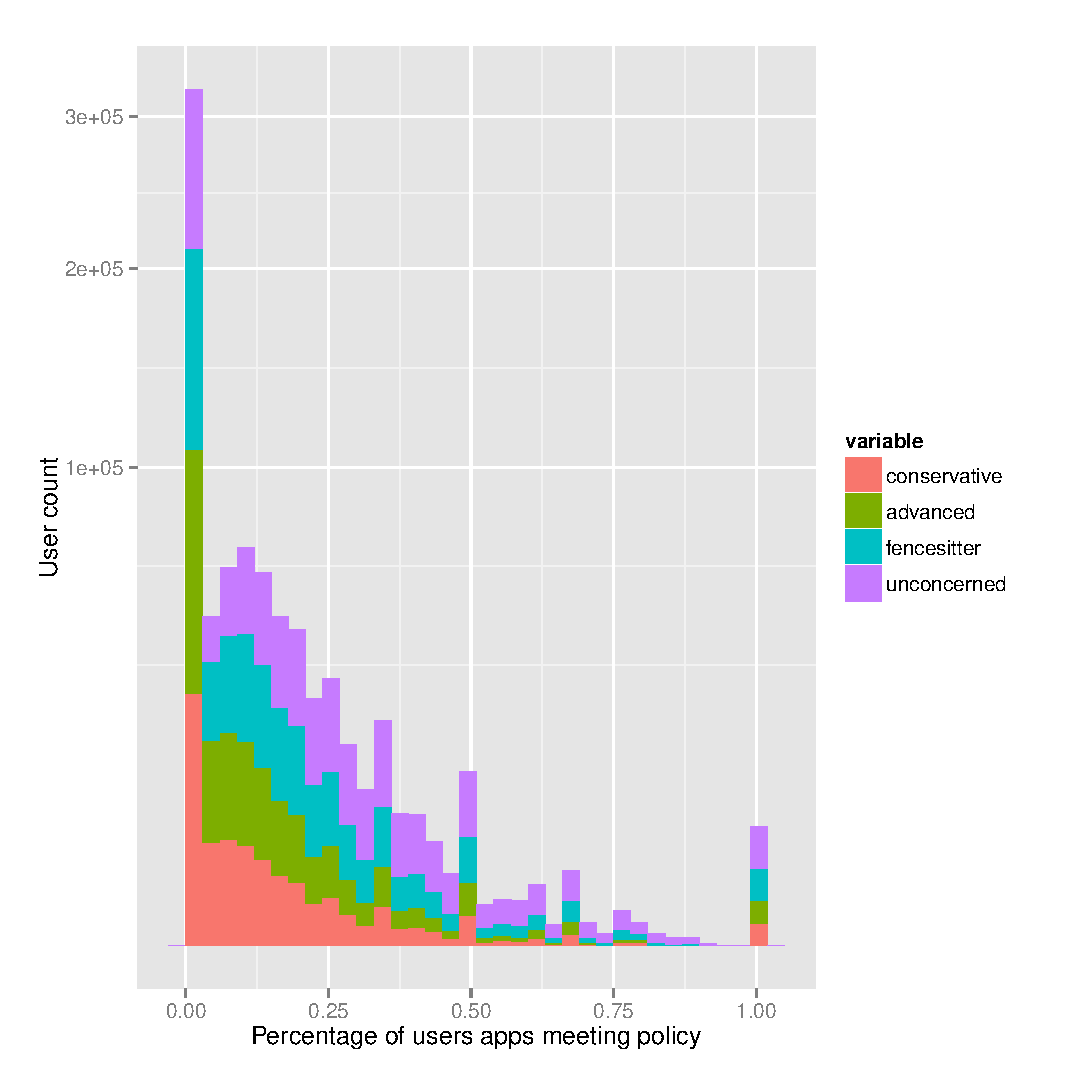
\includegraphics[width=1.0\linewidth]{./tables/lin.eps}
  \caption{Use of policies modelling user behaviour.}
  \label{fig:lin}
\end{figure}

\begin{figure}[!ht]\centering
  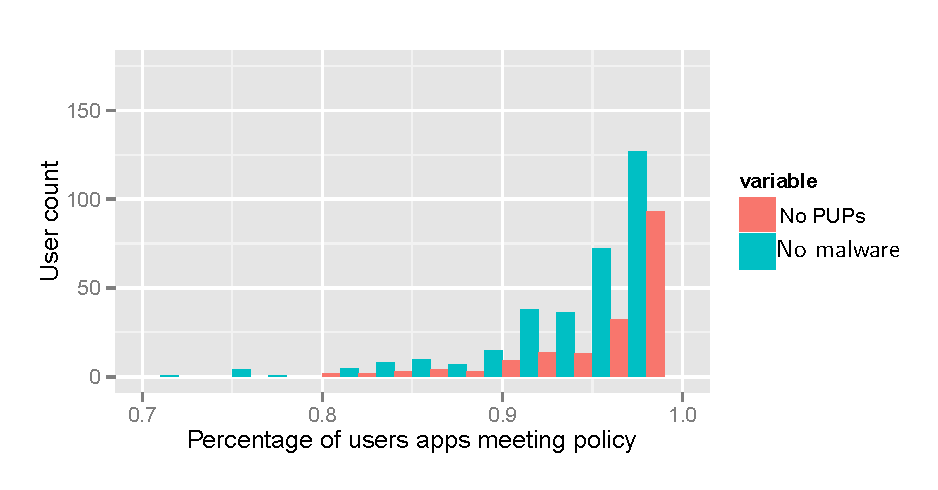
\includegraphics[width=1.0\linewidth]{./tables/malware.eps}
  \caption{Percentage of malware in installed apps for users installing some malicious apps}
  \label{fig:malware}
\end{figure}


In Figure~\ref{fig:lin} we can see that whilst the majority of users rarely
follow these policies there are a few users who do seem to be installing apps on
the basis of these policies most of the time.
This suggests that while users may have privacy preferences the majority are not attempting to enforce them.

We found 2\% of the users had a PUS or malicious app installed.
In Figure~\ref{fig:malware} we see that of those users with a malicious app
installed PUS accounts for around half of the malware infections.

\section{Discussion}

Most users seem to use apps irrespective of how uncomfortable they are with the permissions they request.
A small set of users do seem to enforce these policies at least some of the time however.
Exploring where this disconnect comes from is an avenue for future research.
Do users not understand the relationship between apps and permissions~\citep{Felt:2012hma}.
Is enforcing them too difficult?


AppPAL can capture the differences in user policies.
AppPAL can filter apps on the basis of these policies.  
Using AppPAL we have written short policies describing user behaviour and been able to identify users following them to varying degrees.

Next steps will involve a trial creating an app store for Android with AppPAL
built in.  This will allow us to trial policies with users; and begin testing
more complex policies dynamically.  To begin testing AppPAL we plan an Android
app where a user can check their currently installed apps against several
policies.

\bibliographystyle{plain}
\bibliography{abstract}

\end{document}

